\documentclass{article}
\usepackage[margin=1in]{geometry}
\usepackage{amsmath}
\usepackage{amssymb}
\usepackage{amsthm}
\usepackage{bm}
\usepackage{hyperref}
\usepackage{graphicx}
\usepackage{caption}
\usepackage{listings}
\usepackage{xcolor}
\usepackage{float}
\usepackage{placeins}
\graphicspath{{figures/}}

% Code style
\lstdefinestyle{code}{
  basicstyle=\ttfamily\small,
  numbers=left,
  numberstyle=\tiny,
  numbersep=8pt,
  keywordstyle=\color{blue},
  commentstyle=\color{teal!70!black},
  stringstyle=\color{orange!70!black},
  showstringspaces=false,
  breaklines=true,
  frame=single,
  framerule=0.3pt,
  rulecolor=\color{black!15}
}
\lstset{style=code}

\title{Deep Reinforcement Learning: Value-Based, Policy-Based, and AlphaGo}
\author{}
\date{\today}

\begin{document}
\maketitle
\tableofcontents
\FloatBarrier

\section{DQN, Policy Gradient, and Actor-Critic}
Deep reinforcement learning (DRL) optimizes sequential decision-making policies by combining neural function approximators with RL objectives. Figure~\ref{fig:rl_overview} contrasts key components of value-based, policy-based, and actor-critic algorithms.

\subsection{Deep Q-Network (DQN)}
DQN approximates the optimal action-value function $Q^{\star}(s, a)$ for discrete actions. The Bellman optimality equation states
\begin{equation}
  Q^{\star}(s, a) = \mathbb{E}_{s' \sim P(\cdot \mid s, a)} \left[ r(s, a) + \gamma \max_{a'} Q^{\star}(s', a') \right].
\end{equation}
DQN parameterizes $Q_{\theta}(s, a)$ with a neural network and minimizes the temporal difference (TD) loss:
\begin{equation}
  \mathcal{L}(\theta) = \mathbb{E}_{(s, a, r, s') \sim \mathcal{D}} \left[ \left( y - Q_{\theta}(s, a) \right)^2 \right], \quad y = r + \gamma \max_{a'} Q_{\theta^{-}}(s', a'),
\end{equation}
where $\theta^{-}$ denotes the target network parameters periodically copied from $\theta$. Experience replay $\mathcal{D}$ breaks correlations by sampling uniformly from stored transitions.

\paragraph{Stabilization Techniques}
\begin{itemize}
  \item \textbf{Double DQN:} Replace the $\max$ over target network with $\arg\max$ from the online network to reduce overestimation.
  \item \textbf{Dueling architecture:} Decompose $Q(s, a) = V(s) + A(s, a) - \frac{1}{|\mathcal{A}|} \sum_{a'} A(s, a')$ to capture state values independently.
  \item \textbf{Prioritized replay:} Sample proportional to TD error magnitude to focus on informative transitions.
\end{itemize}

\paragraph{Pseudo-code}
\begin{lstlisting}[language=Python, caption={DQN training loop with target network and replay buffer.}]
replay = ReplayBuffer(capacity=100_000)
q_net = QNetwork().to(device)
target_net = copy.deepcopy(q_net)
optimizer = torch.optim.Adam(q_net.parameters(), lr=1e-3)

for step in range(total_steps):
    action = epsilon_greedy(q_net, obs, epsilon_schedule(step))
    next_obs, reward, done, info = env.step(action)
    replay.add(obs, action, reward, next_obs, done)
    obs = next_obs if not done else env.reset()

    if step > warmup and step % train_freq == 0:
        batch = replay.sample(batch_size=64)
        target = batch.reward + gamma * target_net(batch.next_obs).max(dim=1).values * (1 - batch.done)
        q_values = q_net(batch.obs).gather(1, batch.action.unsqueeze(1)).squeeze(1)
        loss = F.mse_loss(q_values, target.detach())
        optimizer.zero_grad()
        loss.backward()
        clip_grad_norm_(q_net.parameters(), max_norm=10.0)
        optimizer.step()

    if step % target_update == 0:
        target_net.load_state_dict(q_net.state_dict())
\end{lstlisting}

\subsection{Policy Gradient Methods}
Policy gradients maximize expected return $J(\theta) = \mathbb{E}_{\tau \sim \pi_{\theta}} \left[\sum_{t=0}^{T} \gamma^{t} r_t\right]$ with respect to policy parameters $\theta$. The REINFORCE gradient estimator is
\begin{equation}
  \nabla_{\theta} J(\theta) = \mathbb{E}_{\pi_{\theta}} \left[ \sum_{t=0}^{T} \nabla_{\theta} \log \pi_{\theta}(a_t \mid s_t) \, G_t \right], \quad G_t = \sum_{k=t}^{T} \gamma^{k-t} r_k.
\end{equation}
Variance reduction uses baselines $b(s_t)$, yielding
\begin{equation}
  \nabla_{\theta} J(\theta) = \mathbb{E}_{\pi_{\theta}} \left[ \sum_{t} \nabla_{\theta} \log \pi_{\theta}(a_t \mid s_t) \left( G_t - b(s_t) \right) \right].
\end{equation}
Common choices include learned value functions $V_{\phi}(s)$ and advantage estimates $A_t = G_t - V_{\phi}(s_t)$.

\paragraph{Trust Region Policy Optimization (TRPO) and PPO}
TRPO constrains policy updates by the KL divergence between old and new policies. PPO simplifies this with a clipped surrogate objective:
\begin{align}
  L^{\text{CLIP}}(\theta) = \mathbb{E}\left[ \min\left( r_t(\theta) A_t, \operatorname{clip}(r_t(\theta), 1 - \epsilon, 1 + \epsilon) A_t \right) \right], \\
  r_t(\theta) = \frac{\pi_{\theta}(a_t \mid s_t)}{\pi_{\theta_{\text{old}}}(a_t \mid s_t)}.
\end{align}
Generalized advantage estimation (GAE) smooths advantages via $\lambda$-returns:
\begin{equation}
  A_t^{\text{GAE}} = \sum_{l=0}^{\infty} (\gamma \lambda)^l \delta_{t+l}, \quad \delta_t = r_t + \gamma V(s_{t+1}) - V(s_t).
\end{equation}

\subsection{Actor-Critic Frameworks}
Actor-critic methods combine policy (actor) and value (critic) networks. The critic approximates $V_{\phi}(s)$ or $Q_{\phi}(s, a)$ to reduce variance. A2C/A3C perform synchronous/asynchronous updates across multiple workers, while soft actor-critic (SAC) introduces entropy regularization for continuous control:
\begin{equation}
  J_{\pi} = \mathbb{E}_{s_t \sim \mathcal{D}} \left[ \mathbb{E}_{a_t \sim \pi} \left[\alpha \log \pi(a_t \mid s_t) - Q_{\phi}(s_t, a_t)\right] \right],
\end{equation}
where $\alpha$ controls the entropy-temperature trade-off. Deterministic policy gradients (DDPG, TD3) adapt actor-critic to continuous actions via deterministic policies and target smoothing.

\subsection{Comparison Summary}
Figure~\ref{fig:rl_overview} summarizes characteristics:
\begin{itemize}
  \item DQN: discrete actions, off-policy, relies on replay buffer and target network.
  \item Policy gradient: on-policy, handles continuous actions, suffers from high variance without baseline.
  \item Actor-critic: hybrid approach enabling stable updates and continuous control.
\end{itemize}

\begin{figure}[H]
  \centering
  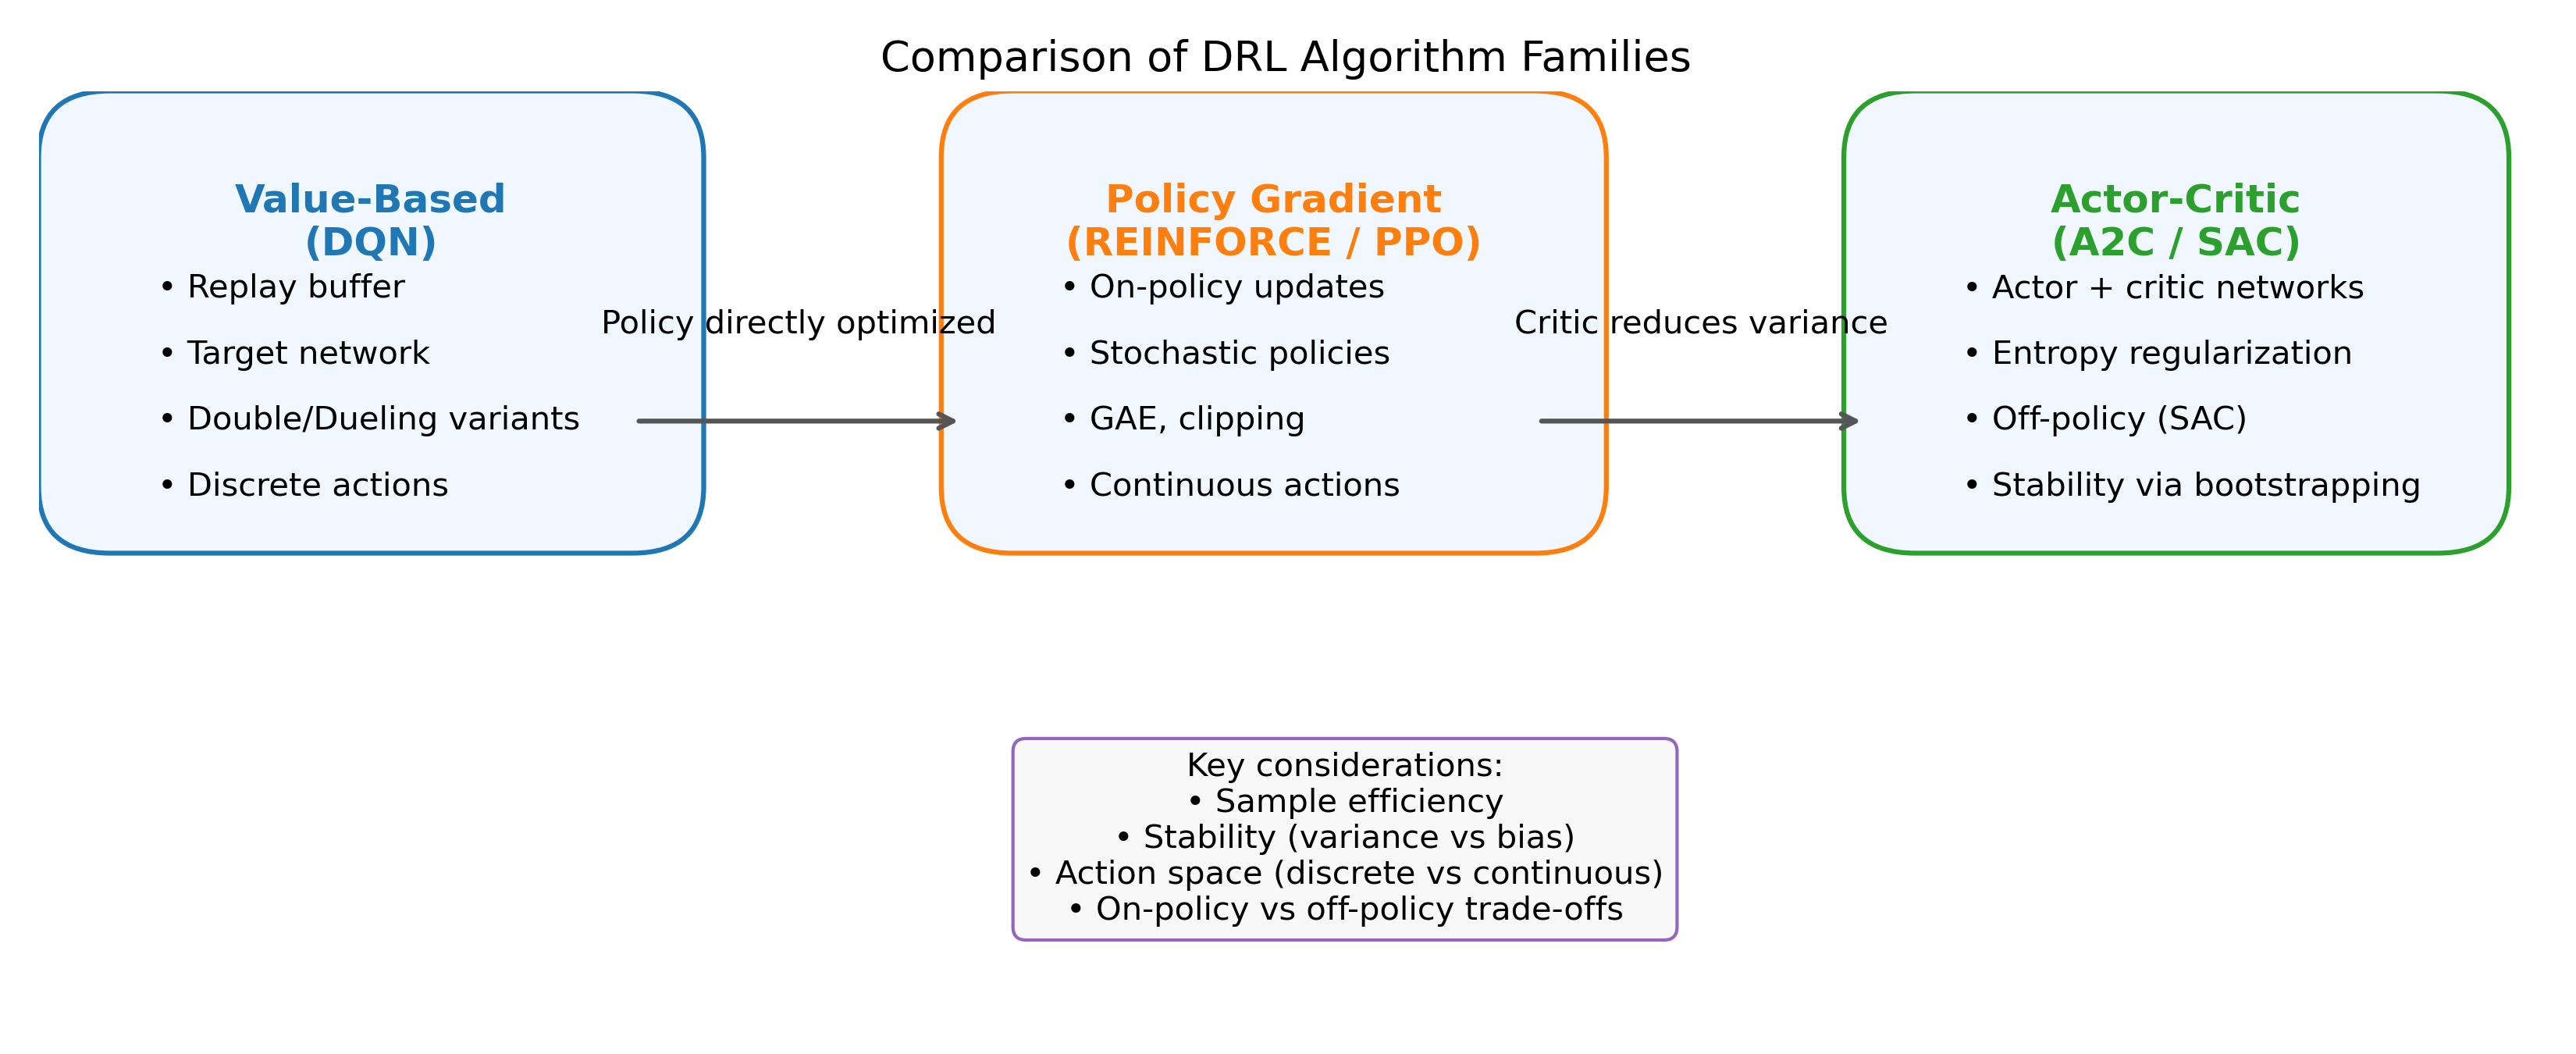
\includegraphics[width=0.9\textwidth]{rl_overview.png}
  \caption{Comparison of DQN, policy gradient, and actor-critic pipelines. Value-based methods rely on replay buffers; policy gradients update policies directly; actor-critic blends both.}
  \label{fig:rl_overview}
\end{figure}
\FloatBarrier

\section{AlphaGo Case Study}
AlphaGo integrates deep learning with Monte Carlo tree search (MCTS), achieving superhuman Go performance. Figure~\ref{fig:alphago_pipeline} shows the training pipeline combining supervised learning (SL), reinforcement learning (RL), and tree search.

\subsection{Policy Network Training}
The supervised policy network $p_{\theta}(a \mid s)$ is trained on expert games via cross-entropy:
\begin{equation}
  \mathcal{L}_{\text{SL}}(\theta) = -\mathbb{E}_{(s, a) \sim \mathcal{D}_{\text{human}}} [\log p_{\theta}(a \mid s)].
\end{equation}
This network initializes a reinforcement learning policy trained by self-play to maximize win rate $\rho(\theta)$ using policy gradient:
\begin{equation}
  \nabla_{\theta} \rho(\theta) = \mathbb{E}_{\tau \sim p_{\theta}} \left[ \left( z - b \right) \sum_{t} \nabla_{\theta} \log p_{\theta}(a_t \mid s_t) \right],
\end{equation}
where $z \in \{-1, +1\}$ is game outcome and $b$ is a baseline to reduce variance.

\subsection{Value Network and Rollouts}
The value network $v_{\phi}(s)$ predicts win probability for state $s$. It is trained on self-play positions with Monte Carlo outcomes $z$:
\begin{equation}
  \mathcal{L}_{\text{value}}(\phi) = \mathbb{E}_{s \sim \mathcal{D}_{\text{self-play}}} \left[ \left( v_{\phi}(s) - z \right)^2 \right].
\end{equation}
During search, fast rollout policies approximate value by simulating random playouts. The blend of value network and rollouts improves evaluation accuracy.

\subsection{Monte Carlo Tree Search Integration}
AlphaGo uses a variant of upper confidence bounds (UCB) for action selection within MCTS:
\begin{equation}
  a_t = \arg\max_{a} \left( Q(s_t, a) + c_{\mathrm{puct}} \, P(s_t, a) \frac{\sqrt{ \sum_b N(s_t, b) }}{1 + N(s_t, a)} \right),
\end{equation}
where $Q$ is mean action value, $P$ prior from the policy network, and $N$ visit counts. The policy and value networks guide tree expansion and evaluation, drastically reducing search space compared to uniform exploration.

\subsection{AlphaGo Zero and AlphaZero}
AlphaGo Zero replaces supervised learning with pure self-play and combines policy/value network into a single residual network outputting $(p, v)$. The training target for policy is visit counts $\pi$ produced by MCTS, while value targets remain game outcomes:
\begin{equation}
  \mathcal{L}(\theta) = (z - v_{\theta}(s))^2 - \pi^{\top} \log p_{\theta}(s) + \lambda \|\theta\|^2.
\end{equation}
AlphaZero generalizes this framework to chess and shogi, demonstrating cross-domain transferability of tree-guided self-play.

\subsection{Engineering Insights}
\begin{itemize}
  \item \textbf{Hardware:} Original AlphaGo used GPU clusters for neural evaluation plus distributed CPUs for MCTS simulations.
  \item \textbf{Training Efficiency:} Replay buffers for self-play games ensure diverse training data; batching tree search evaluations maximizes GPU utilization.
  \item \textbf{Evaluation:} Regimens include Elo rating against previous generations, ablation of components, and match play versus human professionals.
\end{itemize}

\begin{figure}[H]
  \centering
  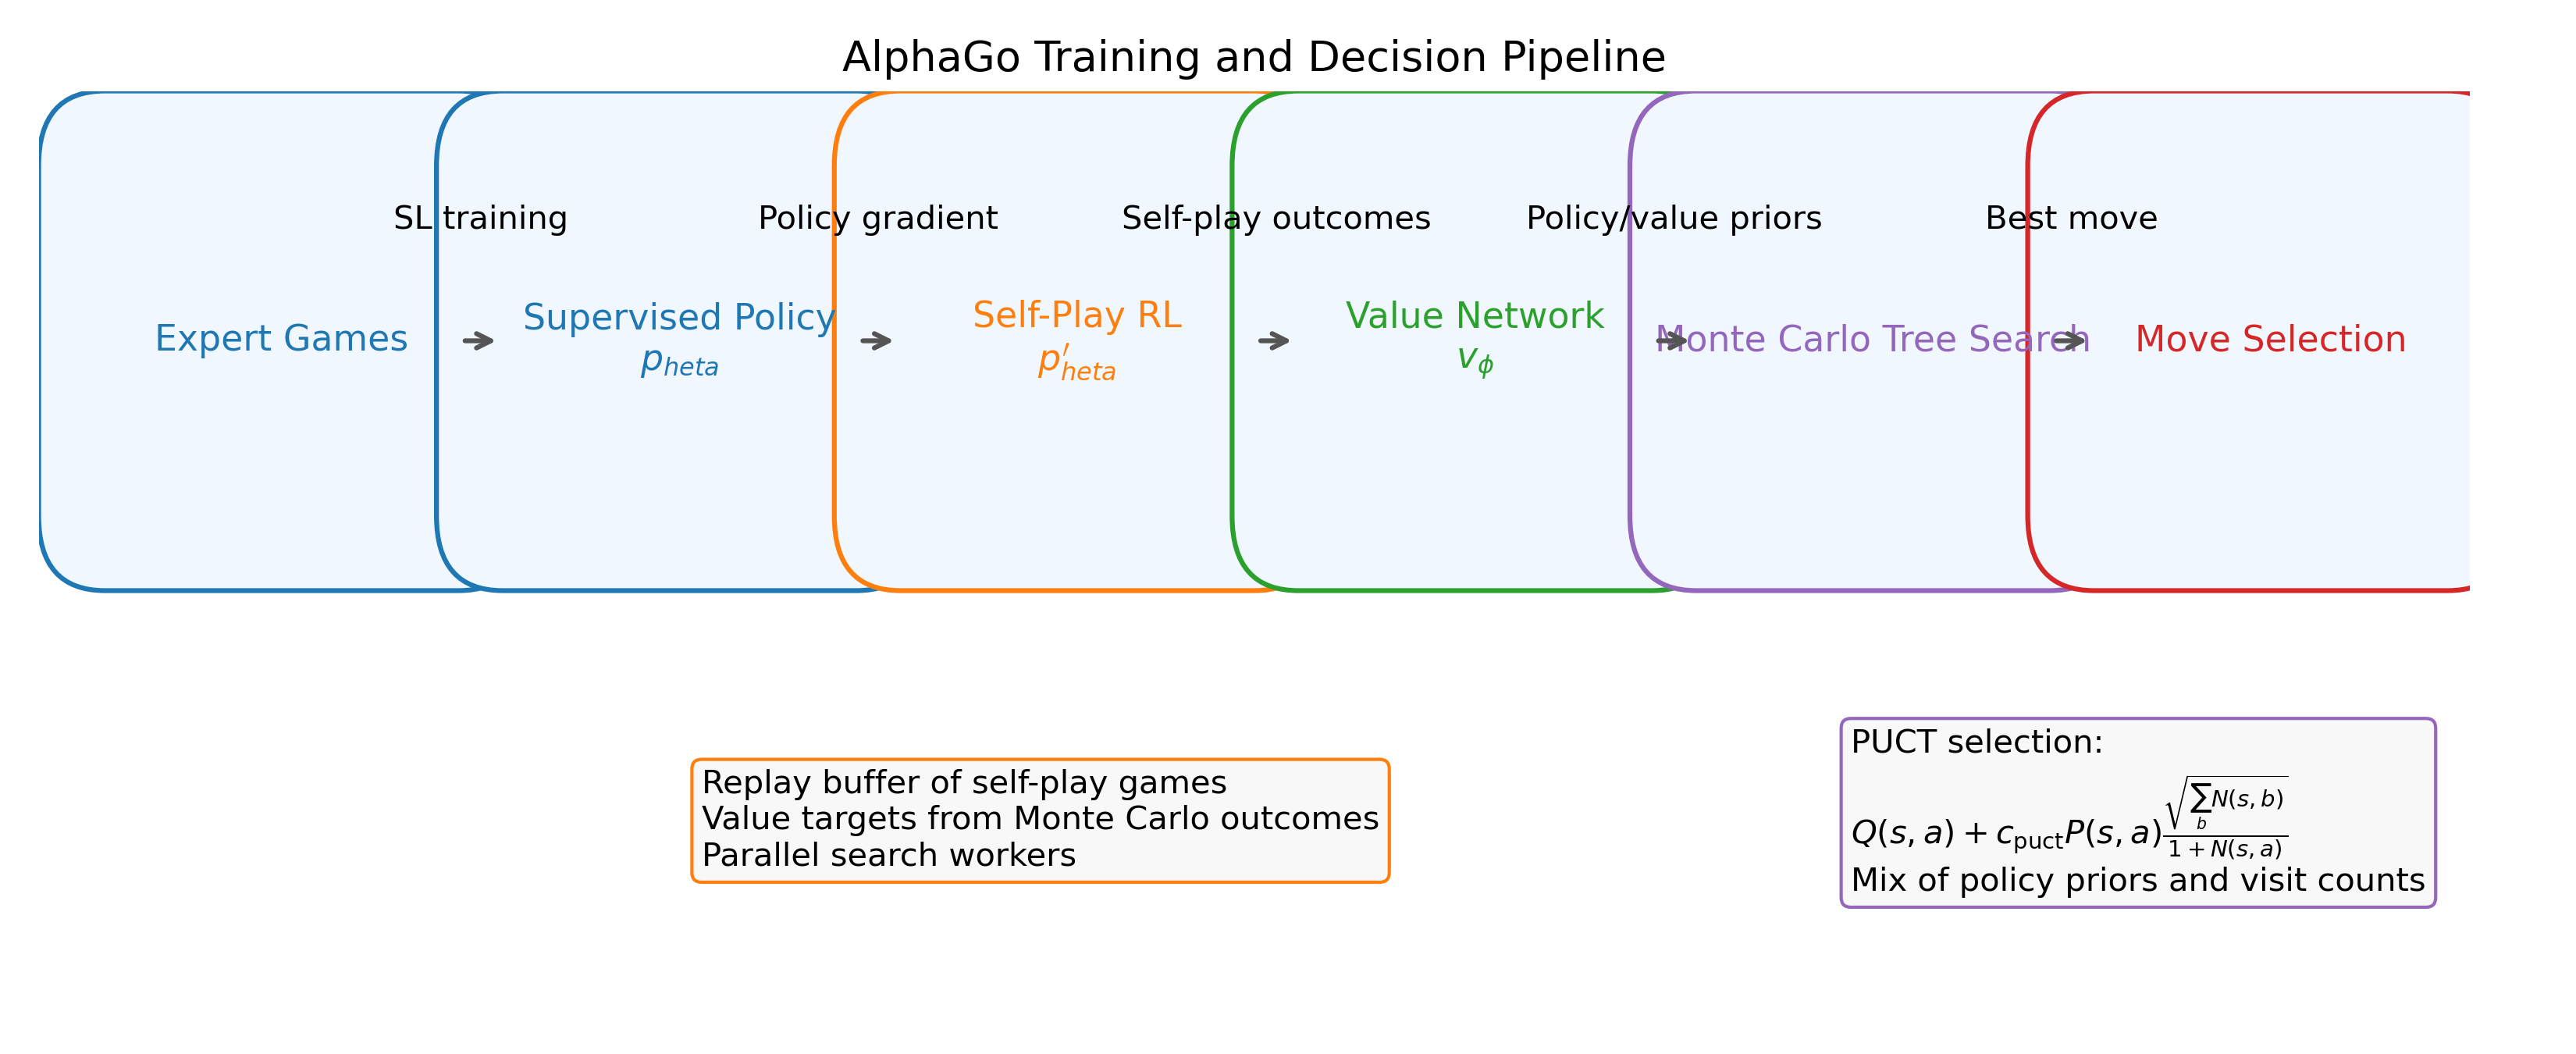
\includegraphics[width=0.9\textwidth]{alphago_pipeline.png}
  \caption{AlphaGo training and inference pipeline: supervised policy initialization, self-play reinforcement learning, value network training, and MCTS-guided decision making.}
  \label{fig:alphago_pipeline}
\end{figure}
\FloatBarrier

\section*{Further Reading}
\begin{itemize}
  \item Volodymyr Mnih et al. ``Playing Atari with Deep Reinforcement Learning.'' NIPS Deep Learning Workshop 2013.
  \item John Schulman et al. ``Proximal Policy Optimization Algorithms.'' arXiv 2017.
  \item Tuomas Haarnoja et al. ``Soft Actor-Critic Algorithms and Applications.'' arXiv 2018.
  \item Silver et al. ``Mastering the game of Go with deep neural networks and tree search.'' Nature 2016.
  \item Silver et al. ``Mastering Chess and Shogi by Self-Play with a General Reinforcement Learning Algorithm.'' arXiv 2017.
\end{itemize}

\end{document}
